\documentclass[a4paper,UTF8,no-math]{ctexart}

%\documentclass[a4paper,UTF8,no-math,zihao=-4]{ctexart}

%\usepackage[backref]{hyperref} 

\usepackage{listings}
\usepackage{wrapfig}
\usepackage{xcolor}

\usepackage{geometry}

\usepackage{zhnumber}

\usepackage{amsmath}% eqref 

\usepackage{amssymb}% mathbb数学符号

\usepackage{algorithm}

\usepackage{algorithmic}

\usepackage{natbib}

\usepackage{multirow}
\usepackage{graphicx}
\usepackage{makecell}

%\usepackage[linkcolor=black,citecolor=blue,anchorcolor=red]{hyperref}

\usepackage{hyperref}

% \usepackage{}

\bibliographystyle{plainnat}



\setmainfont{Times New Roman}

\hypersetup{colorlinks=true}



%\hypersetup{hidelinks,bookmarks=true,bookmarksopen=true}



\geometry{a4paper,left=1.27cm,right=1.27cm,top=1.27cm,bottom=1.27cm}

\lstset{ % General setup for the package
	language=Python,
	numbers=left,
	frame=shadowbox,
	tabsize=4,
	breaklines=true, 
}

\newcommand{\obs}{\text{obs}}
\newcommand{\mis}{\text{mis}}

\newcommand{\qt}[1]{\left<#1\right>}
\newcommand{\ql}[1]{\left[#1\right]}
\newcommand{\hess}{\mathbf{H}}
\newcommand{\jacob}{\mathbf{J}}
\newcommand{\hl}{HL}
\newcommand{\cost}{\mathcal{L}}
\newcommand{\lout}{\mathbf{r}}
\newcommand{\louti}{r}
\newcommand{\outi}{y}
\newcommand{\out}{\mathbf{y}}
\newcommand{\gauss}{\mathbf{G_N}}
\newcommand{\eye}{\mathbf{I}}
\newcommand{\softmax}{\phi}
\newcommand{\targ}{\mathbf{t}}
\newcommand{\metric}{\mathbf{G}}
\newcommand{\sample}{\mathbf{z}}

\newcommand{\bmx}[0]{\begin{bmatrix}}
	\newcommand{\emx}[0]{\end{bmatrix}}
\newcommand{\qexp}[1]{\left<#1\right>}
\newcommand{\vect}[1]{\mathbf{#1}}
\newcommand{\vects}[1]{\boldsymbol{#1}}
\newcommand{\matr}[1]{\mathbf{#1}}
\newcommand{\var}[0]{\operatorname{Var}}
\newcommand{\std}[0]{\operatorname{std}}
\newcommand{\cov}[0]{\operatorname{Cov}}
\newcommand{\diag}[0]{\operatorname{diag}}
\newcommand{\matrs}[1]{\boldsymbol{#1}}
\newcommand{\va}[0]{\vect{a}}
\newcommand{\vb}[0]{\vect{b}}
\newcommand{\vc}[0]{\vect{c}}
\newcommand{\vh}[0]{\vect{h}}
\newcommand{\vv}[0]{\vect{v}}
\newcommand{\vx}[0]{\vect{x}}
\newcommand{\vw}[0]{\vect{w}}
\newcommand{\vs}[0]{\vect{s}}
\newcommand{\vf}[0]{\vect{f}}
\newcommand{\vy}[0]{\vect{y}}
\newcommand{\vg}[0]{\vect{g}}
\newcommand{\vm}[0]{\vect{m}}
\newcommand{\vu}[0]{\vect{u}}
\newcommand{\vL}[0]{\vect{L}}
\newcommand{\mW}[0]{\matr{W}}
\newcommand{\mG}[0]{\matr{G}}
\newcommand{\mX}[0]{\matr{X}}
\newcommand{\mQ}[0]{\matr{Q}}
\newcommand{\mU}[0]{\matr{U}}
\newcommand{\mV}[0]{\matr{V}}
\newcommand{\mA}{\matr{A}}
\newcommand{\mD}{\matr{D}}
\newcommand{\mS}{\matr{S}}
\newcommand{\mI}{\matr{I}}
\newcommand{\td}[0]{\text{d}}
\newcommand{\vsig}[0]{\vects{\sigma}}
\newcommand{\valpha}[0]{\vects{\alpha}}
\newcommand{\vmu}[0]{\vects{\mu}}
\newcommand{\vzero}[0]{\vect{0}}
\newcommand{\tf}[0]{\text{m}}
\newcommand{\tdf}[0]{\text{dm}}
\newcommand{\grad}[0]{\nabla}
\newcommand{\alert}[1]{\textcolor{red}{#1}}
\newcommand{\N}[0]{\mathcal{N}}
\newcommand{\LL}[0]{\mathcal{L}}
\newcommand{\HH}[0]{\mathcal{H}}
\newcommand{\RR}[0]{\mathbb{R}}
\newcommand{\II}[0]{\mathbb{I}}
\newcommand{\Scal}[0]{\mathcal{S}}
\newcommand{\sigmoid}{\sigma}
\newcommand{\E}[0]{\mathbb{E}}
\newcommand{\enabla}[0]{\ensuremath{%
		\overset{\raisebox{-0.3ex}[0.5ex][0ex]{%
				\ensuremath{\scriptscriptstyle e}}}{\nabla}}}
\newcommand{\enhnabla}[0]{\nabla_{\hspace{-0.5mm}e}\,}
\newcommand{\tred}[1]{\textcolor{red}{#1}}
\newcommand{\todo}[1]{{\Large\textcolor{red}{#1}}}
\newcommand{\done}[1]{{\Large\textcolor{green}{#1}}}
\newcommand{\dd}[1]{\ensuremath{\mbox{d}#1}}

\DeclareMathOperator*{\argmax}{\arg \max}
\DeclareMathOperator*{\argmin}{\arg \min}
\newcommand{\newln}{\\&\quad\quad{}}

\newcommand{\Ax}{\mathcal{A}_x}
\newcommand{\Ay}{\mathcal{A}_y}
\newcommand{\ola}{\overleftarrow}
\newcommand{\ora}{\overrightarrow}
\newcommand{\ov}{\overline}

\title{Neural Machine Translation  by Jointly Learning to Align and Translate}

\author{
	Dzmitry Bahdanau \\
	Jacobs University Bremen, Germany
	\and
	KyungHyun Cho~ ~ ~ ~Yoshua Bengio  v  \\
	Universit\'{e} de Montr\'{e}al
}

\date{分享人:高磊 \\ \zhtoday}





\begin{document}
	
	%	\tableofcontents
	%	\newpage
	
	\maketitle
	
	
	\section{提出问题}
	
	近期提出的神经网络机器翻译模型都是encoder-decoder家族的,这些模型把源句子encode成一个定长向量,然后再用一个decoder生成翻译。我们推测使用定长向量是encoder-decoder架构的瓶颈\footnote{《On the properties of neuralmachine translation: Encoder–Decoder approaches》——Cho:随着输入句子变长,encoder-decoder的表现迅速下降}。
	
	
	
	
	\section{解决办法}
	
	
	为此,我们引入了一个扩展的encoder-decoder模型来同时学习对齐(align)和翻译。该模型每次在译文中生成一个词时,都会(软)搜索源句中最相关信息集中的一组位置。然后,该模型根据与这些源位置相关联的上下文向量和所有先前生成的目标词来预测目标词。这个模型把输入的序列encode为一组向量的序列,在decode时自适应地从这组向量序列中选其子集用于翻译。
	
	\begin{wrapfigure}{R}{0.3\textwidth}
		\centering
		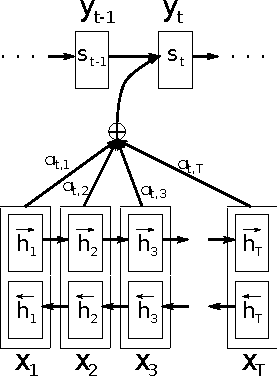
\includegraphics[width=0.29\textwidth]{./images/AttentionMechanism/rnnsearch.pdf}
		\caption{
			图示为在给定源序列$(x_1, x_2,\dots, x_T)$的情况下生成$t$-th目标单词。
		}
		\label{fig:rnnsearch}
	\end{wrapfigure}

	\section{一些细节}
	
	\subsection{ENCODER}
	模型的输入是K维独热向量序列
	\[
	\vx = (x_1, \ldots, x_{T_x}),\mbox{ }x_i \in \mathbb{R}^{K_x}
	\]
	输出是翻译后的K维独热向量序列
	\[
	\vy = (y_1, \ldots, y_{T_y}),\mbox{ }y_i \in \mathbb{R}^{K_y},
	\]
	, $K_x$ 和 $K_y$ 是分别是源语言和目标语言的词表容量。$T_x$ 和 $T_y$ 分别代表原句子和目标句子的长度。
	
	首先,BiRNN的前向状态计算:\begin{align*}
	\ora{h}_i =& 
	\begin{cases}
	(1 - \ora{z}_i) \circ \ora{h}_{i-1}  + \ora{z}_i \circ \ora{\underline{h}}_{i} &\mbox{, if }i > 0 \\
	0 &\mbox{, if }i = 0
	\end{cases}
	\end{align*}其中\begin{align*}
	\ora{\underline{h}}_i =& \tanh \left( \ora{W} \ov{E} x_i + \ora{U}\left[ \ora{r}_i \circ \ora{h}_{i-1} \right] \right) \\
	\ora{z}_i =& \sigma\left( \ora{W}_z \ov{E} x_i + \ora{U}_z \ora{h}_{i-1} \right) \\
	\ora{r}_i =& \sigma\left( \ora{W}_r \ov{E} x_i + \ora{U}_r \ora{h}_{i-1} \right).
	\end{align*}$\overline{E} \in \mathbb{R}^{m\times K_x}$ 是词嵌入矩阵。
	$\ora{W}, \ora{W}_z, \ora{W}_r \in \mathbb{R}^{n\times m}$, $\ora{U}, \ora{U}_z,
	\ora{U}_r \in \mathbb{R}^{n\times n}$ 是权重矩阵。$m$ 和 $n$ 分别是词嵌入维数和隐藏层单元的数量。
	$\sigma(\cdot)$ 是 logistic sigmoid 函数。
	
	BiRNN的反向状态$(\ola{h}_1, \cdots, \ola{h}_{T_x})$的计算方法类似,本文在前向RNN和逆向RNN中共享词嵌入矩阵$\ov{E}$,不共享权重矩阵。
	
	然后把前向和逆向矩阵连接起来得到隐藏状态$(h_1, h_2, \cdots, h_{T_x})$,\begin{align}
	\label{eq:annotation}
	h_i = \left[ 
	\begin{array}{c}
	\ora{h}_i \\
	\ola{h}_i 
	\end{array}
	\right]
	\end{align}
	
	\subsection{DECODER}
	
	给定encoder的隐藏状态的情况下,decoder的隐藏状态$s_i$计算方式为:\begin{align*}
	s_i =& (1 - z_i) \circ s_{i-1} + z_i \circ \tilde{s}_i,
	\end{align*}
	其中
	\begin{align*}
	\tilde{s}_{i} =& \tanh \left( W E y_{i - 1} + U \left[ r_i \circ s_{i - 1} \right] +
	C c_i \right) \\ 
	z_i =& \sigma\left( W_z E y_{i - 1} + U_z s_{i-1} 
	+ C_z c_i \right)\\
	r_i =& \sigma\left( W_r E y_{i - 1} + U_r s_{i-1}
	+ C_r c_i \right)
	\end{align*}$E$ 是目标语言的词向量矩阵。
	$W, W_z, W_r \in \mathbb{R}^{n\times m}$, 
	$U, U_z, U_r \in \mathbb{R}^{n\times n}$, 和
	$C, C_z, C_r \in \mathbb{R}^{n\times 2n}$ 是权重。同样地,$m$ 和 $n$ 分别是词向量矩阵的维数和隐藏单元的数量。初始隐藏状态$s_0$ 计算方式为
	$
	s_{0} = \tanh\left( W_s \ola{h}_1 \right),
	$
	其中 $W_s \in \RR^{n \times n}$。
	
	上下文向量 $c_i$通过对齐模型来计算:
	
	\begin{align*}
	c_i =& \sum_{j=1}^{T_x} \alpha_{ij} h_j,
	\end{align*}
	其中
	\begin{align*}
	\alpha_{ij} =& \frac{\exp\left(e_{ij}\right)}{\sum_{k=1}^{T_x}
		\exp\left(e_{ik}\right)}  \\
	e_{ij} =& v_a^{\top} \tanh\left( W_a s_{i-1} + U_a h_j \right)
	\end{align*}
	并且 $h_j$ 是 $j$-th 源句子的隐藏状态(见Eq.~\eqref{eq:annotation}) 。$v_a \in \mathbb{R}^{n'}, W_a \in
	\mathbb{R}^{n'\times n}$ 和 $U_a \in \mathbb{R}^{n'\times  2n}$ 是权重矩阵。注意:当我们固定$c_i$ 为 $\ora{h}_{T_x}$时,这个模型变成了RNN Encoder--Decoder\footnote{《Learning phrase representations using RNN encoder-decoder for statistical machine translation.》——Cho}。
	
	有了decoder隐藏状态$s_{i-1}$,上下文向量 $c_{i}$ 和上一个生成的单词
	$y_{i-1}$,目标单词  $y_{i}$ 的概率为:
	\begin{align*}
	p(y_{i}|s_i,y_{i-1},c_{i}) \propto& \exp\left(y_{i}^{\top} W_o t_{i}\right),
	\end{align*}
	其中
	\begin{align*}
	t_i =&  \left[ \max\left\{\tilde{t}_{i, 2j-1}, \tilde{t}_{i,2j}\right\}
	\right]_{j=1,\ldots,l}^{\top}
	\end{align*}
	并且 $\tilde{t}_{i,k}$ 是向量$\tilde{t}_i$的 $k$-th 元素,其计算公式为:
	\begin{align*}
	\tilde{t}_{i} =& U_o s_{i - 1} + V_o E y_{i-1} + C_o c_i.
	\end{align*}
	$W_o \in \mathbb{R}^{K_y\times  l}$, $U_o \in \mathbb{R}^{2l\times n}$, $V_o \in
	\mathbb{R}^{2l\times m}$ and $C_o \in \mathbb{R}^{2l\times 2n}$ 是权重矩阵。This can be understood as having a deep output\footnote{《How to construct deep recurrent neural
		networks》——Pascanu}
	with a single maxout hidden layer\footnote{《Maxout net-
		works》——Goodfellow}。
	
	
	
	
	
%	\section{一些细节}
%	
%	\begin{enumerate}
%		\item 模型在找最大概率的翻译时,使用了从左到右的beam search。有趣的是在$ beam size=1 $时,模型也能得到很好的结果、$ beam size =2 $ 的性价比最高,最好的成绩在$ beam size=12 $时取到;
%		\item 初始化LSTM的参数为-0.08到0.08间的均匀分布、固定学习率0.7训练5个epochs,然后每半个epoch减半,共训练7.5epochs、$ batch_size=128 $;
%		\item LSTM没有发生梯度消失,但发生了梯度爆炸,为此使用了梯度裁剪;
%		\item 因为句子有长有短,尽量把长度差不多的句子取在一个batch中,这样避免了算力浪费,平均加速了两倍。
%	\end{enumerate}

\end{document}